% Prezentácia projektu SOUND-EDGE – Metódy inžinierskej práce
% Preklad: pdfLaTeX (2x)

\documentclass[aspectratio=169,11pt]{beamer}

\usepackage[T1]{fontenc}
\usepackage[utf8]{inputenc}
\usepackage[slovak]{babel}
\usepackage[sfdefault,scaled=.92]{FiraSans}
\usepackage{booktabs}
\usepackage{tabularx}
\usepackage{tikz}
\usetikzlibrary{positioning,arrows.meta}

\usetheme[progressbar=frametitle,block=fill,sectionpage=none]{metropolis}

% --- farby šablóny -------------------------------------------------------
\definecolor{seNavy}{HTML}{1F3B57}
\definecolor{seOrange}{HTML}{E07A2E}
\definecolor{seBg}{HTML}{F4F7FB}
\definecolor{seText}{HTML}{23313F}
\definecolor{seGreen}{HTML}{3C8D5A}

\setbeamercolor{normal text}{fg=seText,bg=seBg}
\setbeamercolor{background canvas}{bg=seBg}
\setbeamercolor{frametitle}{fg=white,bg=seNavy}
\setbeamercolor{alerted text}{fg=seOrange}
\setbeamercolor{example text}{fg=seGreen}
\setbeamercolor{progress bar}{fg=seOrange,bg=seNavy!60}
\setbeamercolor{title separator}{fg=seOrange}
\setbeamercolor{block title}{fg=white,bg=seNavy}
\setbeamercolor{block body}{fg=seText,bg=white}
\setbeamercolor{block title alerted}{fg=white,bg=seOrange}
\setbeamercolor{block body alerted}{fg=seText,bg=white}
\setbeamercolor{block title example}{fg=white,bg=seGreen}
\setbeamercolor{block body example}{fg=seText,bg=white}
\setbeamercolor{itemize item}{fg=seOrange}
\setbeamercolor{itemize subitem}{fg=seOrange}
\setbeamercolor{enumerate item}{fg=seOrange}
\setbeamercolor{description item}{fg=seNavy}
\setbeamerfont{description item}{series=\bfseries}
\setbeamerfont{subtitle}{size=\normalsize}
\setbeamertemplate{itemize item}{\small$\blacktriangleright$}

% --- päta s menom prezentujúceho -----------------------------------------
\newcommand{\presenter}{}
\newcommand{\setpresenter}[1]{\renewcommand{\presenter}{#1}}
\setbeamertemplate{footline}{%
  \begin{beamercolorbox}[wd=\paperwidth,ht=3.2ex,dp=1.4ex,leftskip=1.2em,rightskip=1.2em]{footline}%
    \usebeamerfont{page number in head/foot}%
    \textcolor{seNavy}{\textbf{SOUND-EDGE}}%
    \ifx\presenter\empty\else\textcolor{seText!70}{\quad·\quad\presenter}\fi
    \hfill\textcolor{seText!70}{\insertframenumber\,/\,\inserttotalframenumber}%
  \end{beamercolorbox}}

% --- vlastná úvodná snímka časti (tmavé pozadie + prezentujúci) ----------
\AtBeginSection[]{%
  {\setbeamercolor{background canvas}{bg=seNavy}%
   \begin{frame}[plain,noframenumbering]
     \vfill
     {\color{seOrange}\rule{3em}{2pt}}\par\medskip
     {\color{white}\LARGE\bfseries\insertsectionhead}\par\medskip
     {\color{white!75}\large Prezentuje: \presenter}
     \vfill
   \end{frame}}}

\newcommand{\zdroj}[1]{\par\vfill\hfill{\scriptsize\color{seText!65}#1}}

% --- titulná snímka ------------------------------------------------------
\title{SOUND-EDGE}
\subtitle{Akustická prediktívna údržba priemyselných zariadení\\pomocou okrajového strojového učenia a IoT}
\author{Gabriela Tovarňáková \quad Pavel Ustimenko \quad Ján Vargovčík}
\institute{Fakulta informatiky a informačných technológií STU v Bratislave}
\date{Metódy inžinierskej práce \quad·\quad 2026/2027 \quad·\quad vedenie: Ing. Ivan Kapustík}

\begin{document}

{\setbeamercolor{background canvas}{bg=seNavy}
 \setbeamercolor{normal text}{fg=white}
 \setbeamercolor{title}{fg=white}
 \setbeamercolor{subtitle}{fg=white!85}
 \setbeamercolor{author}{fg=white}
 \setbeamercolor{institute}{fg=white!75}
 \setbeamercolor{date}{fg=white!75}
 \usebeamercolor[fg]{normal text}
 \begin{frame}[plain,noframenumbering]
   \titlepage
 \end{frame}}

% =========================================================================
\begin{frame}{Obsah prezentácie}
  \begin{columns}[T]
    \begin{column}{0.48\textwidth}
      \begin{enumerate}
        \item Motivácia a problém
        \item Stav poznania a ciele projektu
        \item Návrh riešenia a merateľné ukazovatele
        \item Realizácia, prínosy a otvorené otázky
      \end{enumerate}
    \end{column}
    \begin{column}{0.48\textwidth}
      \begin{block}{Prezentujú}
        \begin{description}[Gabriela T.]
          \item[Ján V.] časti 1 a 4
          \item[Pavel U.] časť 2
          \item[Gabriela T.] časť 3
        \end{description}
      \end{block}
    \end{column}
  \end{columns}
\end{frame}

% =========================================================================
\setpresenter{Ján Vargovčík}
\section{Motivácia a problém}

\begin{frame}{Prečo prediktívna údržba?}
  \begin{columns}[T]
    \begin{column}{0.52\textwidth}
      \begin{itemize}
        \item Neplánovaná odstávka stroja patrí v priemysle k najdrahším udalostiam.
        \item Údržba sa posúva od \emph{opravy po poruche} cez \emph{pravidelné intervaly} k \alert{prediktívnej údržbe} -- zásah podľa aktuálneho stavu stroja \cite{njor}.
        \item Stav rotujúcich strojov (motory, čerpadlá, ventilátory) najlepšie prezrádzajú \textbf{vibrácie a zvuk}.
      \end{itemize}
    \end{column}
    \begin{column}{0.44\textwidth}
      \begin{alertblock}{Problém dnešných riešení}
        Surový signál sa posiela do cloudu:
        \begin{itemize}
          \item asi \textbf{3,46 GB za deň} z jedného senzora,
          \item zaťaženie siete a oneskorenie,
          \item citlivé dáta opúšťajú podnik,
          \item komerčné systémy sú drahé pre malé a stredné podniky.
        \end{itemize}
      \end{alertblock}
    \end{column}
  \end{columns}
\end{frame}

\begin{frame}{Ako sa porucha prejaví v signáli?}
  \begin{itemize}
    \item Najčastejšie zlyhávajú \textbf{valivé ložiská}. Drobné poškodenie vyvolá pri každom prechode valivého telesa krátky náraz, ktorý sa pravidelne opakuje \cite{randall}.
    \item V počiatočnom štádiu sú nárazy slabé a prekrýva ich hluk stroja.
  \end{itemize}
  \medskip
  \begin{columns}[T]
    \begin{column}{0.47\textwidth}
      \begin{block}{Vibrácie -- akcelerometer}
        \begin{itemize}
          \item pripevnený priamo na stroj
          \item presný signál z jedného miesta
        \end{itemize}
      \end{block}
    \end{column}
    \begin{column}{0.47\textwidth}
      \begin{block}{Zvuk -- mikrofón}
        \begin{itemize}
          \item bez kontaktu, aj viac strojov naraz
          \item citlivejší na okolitý hluk \cite{dcase}
        \end{itemize}
      \end{block}
    \end{column}
  \end{columns}
  \medskip
  \centering\alert{Oba signály sa dopĺňajú $\Rightarrow$ projekt ich plánuje kombinovať.}
\end{frame}

\begin{frame}{Dostupné dáta}
  \small
  \begin{tabularx}{\textwidth}{@{}l l >{\raggedright\arraybackslash}X >{\raggedright\arraybackslash}X@{}}
    \toprule
    \textbf{Dataset} & \textbf{Signál} & \textbf{Obsah} & \textbf{Využitie v projekte} \\
    \midrule
    NASA IMS \cite{nasa} & vibrácie & 4 ložiská na spoločnom hriadeli bežia pod záťažou až do zlyhania & sledovanie postupného opotrebenia \\
    \addlinespace
    MIMII \cite{mimii} & zvuk & nahrávky skutočných priemyselných strojov aj s hlukom prevádzky & detekcia akustických anomálií \\
    \addlinespace
    ToyADMOS \cite{toyadmos} & zvuk & zvuky zmenšených modelov strojov & doplnkové zvukové dáta \\
    \bottomrule
  \end{tabularx}
  \normalsize
  \smallskip
  \begin{exampleblock}{Spôsob vyhodnotenia podľa súťaže DCASE 2020 \cite{dcase}}
    Model sa trénuje iba na zvukoch zdravých strojov. Hodnotí sa, ako dobre odlíši zdravý zvuk od poruchového -- plochou pod ROC krivkou \textbf{(AUC)}: 1 = dokonalé rozlíšenie, 0,5 = náhodný odhad.
  \end{exampleblock}
\end{frame}

% =========================================================================
\setpresenter{Pavel Ustimenko}
\section{Stav poznania a ciele projektu}

\begin{frame}{Detekcia anomálií: učíme sa iba zdravý stroj}
  \begin{columns}[c]
    \begin{column}{0.5\textwidth}
      \begin{itemize}
        \item Dát o skutočných poruchách je málo \cite{lei}.
        \item \textbf{Autoenkodér} -- neurónová sieť, ktorá vstup skomprimuje a znova zrekonštruuje.
        \item Trénuje sa iba na zdravých dátach, poruchový signál preto zrekonštruuje horšie.
        \item Referenčné riešenie DCASE 2020 \cite{dcase} je práve autoenkodér nad spektrogramom.
      \end{itemize}
    \end{column}
    \begin{column}{0.46\textwidth}
      \begin{block}{Skóre anomálie}
        \[
          s(\mathbf{x}) = \frac{1}{N}\sum_{i=1}^{N}\left(x_i-\hat{x}_i\right)^2
        \]
        \small $x_i$ -- vstup, $\hat{x}_i$ -- rekonštrukcia.\\
        Ak $s(\mathbf{x})$ prekročí prah $\Rightarrow$ \alert{anomália}.
      \end{block}
    \end{column}
  \end{columns}
\end{frame}

\begin{frame}{TinyML: strojové učenie priamo na mikrokontroléri}
  \begin{columns}[T]
    \begin{column}{0.5\textwidth}
      \begin{itemize}
        \item Okrajové výpočty (\emph{edge computing}) spracúvajú dáta tam, kde vznikajú \cite{shi}.
        \item Mikrokontrolér: desiatky až stovky kB pamäte, spotreba niekoľko mW \cite{njor}.
        \item Dáta, model, softvérový rámec a hardvér treba navrhovať \textbf{spoločne} \cite{njor}.
      \end{itemize}
    \end{column}
    \begin{column}{0.46\textwidth}
      \begin{block}{Kvantizácia \cite{jacob}}
        32-bitové desatinné čísla $\rightarrow$ 8-bitové celé čísla\\
        $\Rightarrow$ model asi \textbf{4$\times$ menší} a rýchlejší.
      \end{block}
      \begin{block}{MLPerf Tiny \cite{mlperf}}
        Benchmark meria presnosť, rýchlosť aj spotrebu. Obsahuje aj detekciu anomálií vo zvuku strojov.
      \end{block}
    \end{column}
  \end{columns}
\end{frame}

\begin{frame}{Otvorené problémy}
  \begin{enumerate}
    \item \textbf{Oddelený vývoj.} Vibračná diagnostika \cite{lei} a akustická detekcia \cite{dcase} sa vyvíjajú na rôznych dátach a s rôznymi metrikami. Kombináciu na mikrokontroléri sme nenašli.
    \medskip
    \item \textbf{Málo dát o poruchách.} Modely sa ťažko prenášajú medzi strojmi \cite{lei}.
    \medskip
    \item \textbf{Chýba hodnotenie nasaditeľnosti.} Mnohé práce uvádzajú iba presnosť, nie pamäť a rýchlosť \cite{njor,mlperf}.
  \end{enumerate}
\end{frame}

\begin{frame}{Ciele projektu}
  \begin{block}{Hlavný cieľ}
    Navrhnúť a simulačne overiť architektúru a modely, ktoré na lacnom mikrokontroléri v reálnom čase odhalia začínajúce poruchy ložísk a motorov zo zvuku a vibrácií -- \alert{bez posielania surových dát do cloudu}.
  \end{block}
  \medskip
  \begin{description}[C4]
    \item[C1] architektúra zariadenia od snímania signálu po odoslanie výsledku
    \item[C2] malé modely detekcie anomálií pre vibrácie aj zvuk a ich kombinácia
    \item[C3] optimalizácia pre mikrokontrolér (kvantizácia) bez veľkej straty úspešnosti
    \item[C4] vyhodnotenie na verejných datasetoch so správne oddelenými dátami
  \end{description}
\end{frame}

% =========================================================================
\setpresenter{Gabriela Tovarňáková}
\section{Návrh riešenia a merateľné ukazovatele}

\begin{frame}{Architektúra systému SOUND-EDGE}
  \centering
  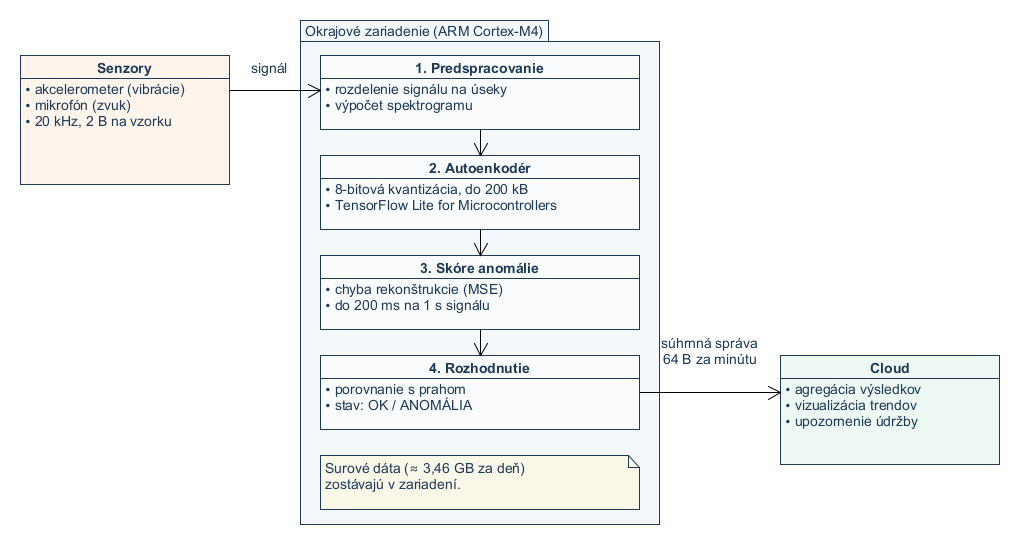
\includegraphics[height=0.76\textheight]{architektura.png}
  \zdroj{Diagram: UMLet (architektura.uxf)}
\end{frame}

\begin{frame}{Metodika overenia}
  \centering
  \begin{tikzpicture}[
      node distance=0.4cm,
      box/.style={draw=seNavy, fill=white, rounded corners=3pt, line width=0.8pt,
                  text width=2.15cm, minimum height=1.6cm, align=center, font=\footnotesize,
                  execute at begin node={\hyphenpenalty=10000\relax}},
      hl/.style={box, fill=seOrange!15, draw=seOrange},
      arr/.style={-{Stealth[length=2.5mm]}, line width=1pt, seNavy}]
    \node[box] (d) {\textbf{Dáta}\\NASA IMS,\\MIMII,\\ToyADMOS};
    \node[box, right=of d] (r) {\textbf{Referencie}\\prah na RMS,\\autoenkodér\\DCASE};
    \node[box, right=of r] (m) {\textbf{Vlastné\\modely}\\vibrácie, zvuk,\\kombinácia};
    \node[hl,  right=of m] (q) {\textbf{Kvantizácia}\\8-bit,\\TF Lite Micro};
    \node[box, right=of q] (e) {\textbf{Hodnotenie}\\AUC, pamäť,\\čas,\\prenos dát};
    \draw[arr] (d) -- (r);
    \draw[arr] (r) -- (m);
    \draw[arr] (m) -- (q);
    \draw[arr] (q) -- (e);
  \end{tikzpicture}
  \bigskip
  \begin{itemize}
    \item Trénovacie a testovacie dáta budú oddelené aj časovo, aby nedošlo k úniku informácií.
    \item Čas spracovania sa bude merať v \textbf{emulácii} mikrokontroléra, nie na fyzickom zariadení.
    \item Podľa vzoru MLPerf Tiny \cite{mlperf} sa okrem úspešnosti uvedie aj pamäť a rýchlosť.
  \end{itemize}
\end{frame}

\begin{frame}{Merateľné ukazovatele}
  \begin{tabularx}{\textwidth}{@{}>{\raggedright\arraybackslash}X l >{\raggedright\arraybackslash}X@{}}
    \toprule
    \textbf{Ukazovateľ} & \textbf{Cieľová hodnota} & \textbf{Spôsob overenia} \\
    \midrule
    AUC detekcie (MIMII, ToyADMOS) & \alert{+10 p.\,b.} oproti DCASE & postup súťaže DCASE 2020 \\
    Pokles AUC po kvantizácii & \alert{najviac 2 p.\,b.} & pôvodný vs. kvantizovaný model \\
    Veľkosť modelu & \alert{do 200 kB} & údaje z prekladu modelu \\
    Čas spracovania 1 s signálu & \alert{do 200 ms} & emulácia mikrokontroléra \\
    Úspora prenášaných dát & \alert{aspoň 99,9 \%} & vzťah pre $\eta$ (ďalšia snímka) \\
    \bottomrule
  \end{tabularx}
  \zdroj{p.\,b. -- percentuálne body; hodnoty sú cieľové odhady tímu}
\end{frame}

\begin{frame}{Koľko dát ušetríme?}
  \begin{columns}[c]
    \begin{column}{0.4\textwidth}
      \[ \eta = 1 - \frac{m \cdot k}{f_s \cdot b \cdot T} \]
    \end{column}
    \begin{column}{0.56\textwidth}
      \scriptsize
      $f_s$ -- vzorkovacia frekvencia, $b$ -- bajty na vzorku,\\
      $T$ -- obdobie (1 deň), $m$ -- veľkosť správy (64 B),\\
      $k$ -- počet správ za obdobie
    \end{column}
  \end{columns}
  \medskip
  \footnotesize
  \setlength{\tabcolsep}{3.5pt}
  \begin{tabularx}{\textwidth}{@{}>{\raggedright\arraybackslash}X r r r r r c@{}}
    \toprule
    \textbf{Scenár} & $f_s$ & \textbf{Interval} & \textbf{Surové} & \textbf{Odoslané} & $\eta$ & \textbf{Cieľ} \\
    \midrule
    Vibrácie, správa za minútu        & 20 kHz   & 60 s    & 3,456 GB & 92,16 kB     & 99,997 \% & \textcolor{seGreen}{áno} \\
    Vibrácie, správa za sekundu       & 20 kHz   & 1 s     & 3,456 GB & 5 529,60 kB  & 99,840 \% & \textcolor{seOrange}{nie} \\
    Zvuk 16 kHz, správa za minútu     & 16 kHz   & 60 s    & 2,765 GB & 92,16 kB     & 99,997 \% & \textcolor{seGreen}{áno} \\
    Zvuk 44,1 kHz, správa každých 10 s & 44,1 kHz & 10 s    & 7,620 GB & 552,96 kB    & 99,993 \% & \textcolor{seGreen}{áno} \\
    Vibrácie, správa každých 10 ms    & 20 kHz   & 0,01 s  & 3,456 GB & 552 960 kB   & 84,000 \% & \textcolor{seOrange}{nie} \\
    \bottomrule
  \end{tabularx}
  \normalsize
  \medskip

  Objemy sú za jeden deň. Cieľ 99,9 \% sa splní, ak zariadenie posiela súhrnnú správu najviac raz za niekoľko sekúnd.
  \zdroj{Tabuľka: MS Excel (uspora\_dat.xlsx), hodnoty počítané vzorcom}
\end{frame}

% =========================================================================
\setpresenter{Ján Vargovčík}
\section{Realizácia, prínosy a otvorené otázky}

\begin{frame}{Harmonogram a rozpočet}
  \begin{columns}[T]
    \begin{column}{0.55\textwidth}
      \begin{block}{Tri etapy (07/2027 -- 06/2030)}
        \begin{description}[07/2029]
          \item[07/2027] analýza datasetov, návrh architektúry, referenčné metódy
          \item[07/2028] vývoj modelov TinyML a ich kvantizácia
          \item[07/2029] simulačné overenie a vyhodnotenie ukazovateľov
        \end{description}
      \end{block}
    \end{column}
    \begin{column}{0.41\textwidth}
      \small
      \begin{tabularx}{\textwidth}{@{}X r@{}}
        \toprule
        \textbf{Položka} & \textbf{EUR} \\
        \midrule
        Mzdy (1 200 h) & 22 500 \\
        Odvody (34 \%) & 7 650 \\
        Materiál, služby & 9 000 \\
        Cestovné, energie & 3 600 \\
        Popularizácia & 1 000 \\
        Nepriame náklady (20 \%) & 8 750 \\
        \midrule
        \textbf{Spolu z APVV} & \textbf{52 500} \\
        \bottomrule
      \end{tabularx}
    \end{column}
  \end{columns}
\end{frame}

\begin{frame}{Prínosy a otvorené otázky}
  \begin{columns}[T]
    \begin{column}{0.48\textwidth}
      \begin{exampleblock}{Očakávané prínosy}
        \begin{itemize}
          \item posun z TRL 2 na \textbf{TRL 3} -- experimentálne overený koncept
          \item prediktívna údržba dostupná aj pre malé a stredné podniky
          \item citlivé dáta zostanú v podniku
          \item menej prenosu dát $\Rightarrow$ nižšia spotreba energie
        \end{itemize}
      \end{exampleblock}
    \end{column}
    \begin{column}{0.48\textwidth}
      \begin{alertblock}{Čo zostáva otvorené}
        \begin{itemize}
          \item datasety nemajú súčasné zvukové a vibračné merania toho istého stroja
          \item simulácia nemusí presne zodpovedať reálnemu hardvéru
          \item prenos modelov medzi rôznymi strojmi
        \end{itemize}
      \end{alertblock}
    \end{column}
  \end{columns}
\end{frame}

\begin{frame}{Zhrnutie}
  \begin{itemize}
    \item SOUND-EDGE spojí vibračnú diagnostiku, akustickú detekciu anomálií a TinyML.
    \item Lacný mikrokontrolér bude porovnávať signál so správaním zdravého stroja a do cloudu pošle iba výsledok.
    \item Riešenie bude overené na verejných datasetoch podľa merateľných ukazovateľov.
  \end{itemize}
  \bigskip
  \centering
  {\Large\color{seNavy}\textbf{Ďakujeme za pozornosť}}\par\smallskip
  {\color{seText!70}Tešíme sa na vaše otázky.}
\end{frame}

\setbeamertemplate{bibliography item}[text]
\setbeamerfont{bibliography item}{size=\scriptsize}
\setbeamerfont{bibliography entry author}{size=\scriptsize}
\setbeamerfont{bibliography entry title}{size=\scriptsize}
\setbeamerfont{bibliography entry location}{size=\scriptsize}
\setbeamerfont{bibliography entry note}{size=\scriptsize}
\begin{frame}{Použité zdroje}
  \scriptsize
  \begin{thebibliography}{10}
    \bibitem{njor} E. Njor, M. A. Hasanpour, J. Madsen, X. Fafoutis. A Holistic Review of the TinyML Stack for Predictive Maintenance. \emph{IEEE Access}, 12, 2024.
    \bibitem{lei} Y. Lei a kol. Applications of machine learning to machine fault diagnosis: A review and roadmap. \emph{Mechanical Systems and Signal Processing}, 138, 2020.
    \bibitem{randall} R. B. Randall, J. Antoni. Rolling element bearing diagnostics -- A tutorial. \emph{Mechanical Systems and Signal Processing}, 25(2), 2011.
    \bibitem{nasa} J. Lee, H. Qiu, G. Yu, J. Lin. Bearing Data Set. NASA Prognostics Data Repository, 2007.
    \bibitem{mimii} H. Purohit a kol. MIMII Dataset: Sound Dataset for Malfunctioning Industrial Machine Investigation and Inspection. \emph{DCASE 2019 Workshop}, 2019.
    \bibitem{toyadmos} Y. Koizumi a kol. ToyADMOS: A Dataset of Miniature-Machine Operating Sounds for Anomalous Sound Detection. \emph{IEEE WASPAA}, 2019.
    \bibitem{dcase} Y. Koizumi a kol. Description and Discussion on DCASE2020 Challenge Task2. \emph{DCASE 2020 Workshop}, 2020.
    \bibitem{shi} W. Shi a kol. Edge Computing: Vision and Challenges. \emph{IEEE Internet of Things Journal}, 3(5), 2016.
    \bibitem{jacob} B. Jacob a kol. Quantization and Training of Neural Networks for Efficient Integer-Arithmetic-Only Inference. \emph{CVPR}, 2018.
    \bibitem{mlperf} C. Banbury a kol. MLPerf Tiny Benchmark. \emph{NeurIPS Datasets and Benchmarks}, 2021.
  \end{thebibliography}
\end{frame}

\end{document}
